\documentclass[11pt]{article}
\usepackage[]{acl}
\usepackage{times}
\usepackage{latexsym}
\usepackage[T1]{fontenc}
\usepackage[utf8]{inputenc}
\usepackage{microtype}
\usepackage{inconsolata}
\usepackage{booktabs}
\usepackage{graphicx}
\usepackage{amsmath}
\usepackage{multirow}

\title{Steering with Empathy: Analysing LLM Behaviour under\\Human User Emotional State}

\author{Sri Charan Sripadi \And Procheta Sen \And Danushka Bollegala}

\newcommand{\todo}[1]{\textbf{[#1]}}

\begin{document}
\maketitle

\begin{abstract}
Human users interact with Large Language Model (LLM)-based agents using textual instructions. In doing so, they express complex and diverse emotions within their prompts, expecting the LLM to understand and respond accordingly. Prior work on how LLMs are influenced by the emotion a user expresses in the prompt is contradictory: some report that task performance is unaffected, others report clear effects. We revisit this question with six families of emotional prefixes (career pressure, reward, a warning to be careful, an expert role with high stakes, threat, and a carefree low-pressure framing), each at three intensities and four wordings, on four tasks and three LLMs (Qwen3-1.7B, Qwen3-8B, Llama-3.2-3B-Instruct). Emotional prefixes change accuracy by only a few points on commonsense and social reasoning, but a carefree framing collapses arithmetic reasoning on GSM8K for all three models (by 35 to 71 points), and some prefixes cause large drops on specific model--task pairs. To look inside the models, we compare the sparse-autoencoder (SAE) features that different prefixes activate at a probing-selected layer. In four of six model--task cells, a prefix framing overlaps with the neutral framing much less than two different questions do, but plain rewordings of the neutral prompt produce the same drop: in 31 of 36 model--task--emotion comparisons the overlap lies inside the range obtained by rewording alone. Feature overlap therefore cannot separate emotion from prompt wording, and we report this negative result together with the one lead that survives the control.
\end{abstract}

\section{Introduction}

LLMs are now widely used to make predictions and evaluations in NLP applications \citep{zhao2023survey}. Human performance is known to depend on emotional state \citep{yerkes1908}, and users routinely express emotion when they address an LLM, for example by stressing that an answer matters to their career, by promising a reward, or by threatening to switch the model off. Whether the performance of LLMs is affected in the same way is unsettled. Several papers report that emotional or social framing changes accuracy \citep{li2023emotion,dobariya2025mind,kuznetsov2026freakout}, while others find that the effect is weak or input dependent \citep{zhao2026emotions}. The answer to the question of whether LLMs are affected by the emotion expressed in the instruction therefore remains inconclusive. In this paper we investigate it using multiple LLMs, tasks and emotion types, and we ask a second question that earlier work leaves open: if behaviour changes, can the change be seen in the model's internal representations, and can it be attributed to emotion rather than to the particular words of the prompt? Throughout, \emph{user emotion} is short for the emotion expressed by the user to an LLM in the prompt.

\paragraph{Behavioural findings.} We evaluate three LLMs on GSM8K, CommonsenseQA, Social IQa and the low-ambiguity part of MoralChoice, with 84 prefixes per dataset. The effect of user emotion depends strongly on the task and, to a lesser degree, on the model. On CommonsenseQA and Social IQa all prefixes stay within about three points of the neutral prompt for every model. On GSM8K and on MoralChoice for the smallest model, some prefixes cause large drops. The clearest case is the carefree framing, which lowers GSM8K accuracy by 35.2, 68.3 and 70.6 points for Qwen3-1.7B, Qwen3-8B and Llama-3.2-3B. The largest model reaches 100\% on low-ambiguity MoralChoice under every framing, so capability can remove the sensitivity entirely on an easy task.

\paragraph{Mechanistic findings.} To study whether the influence is localised in the model, we use sparse autoencoders \citep{cunningham2024sae,bricken2023monosemanticity}. For each model--task pair we choose one layer by probing, encode the last-token residual stream with a pretrained SAE, and measure the overlap of the active feature sets between framings. Overlap between the same question under a prefix and under the neutral prompt is far lower than overlap between two different questions in most cells, which could be read as an emotion effect. A wording control removes that reading: rewording the neutral prompt, with no emotion at all, lowers overlap just as much. In 31 of 36 comparisons the emotion framing lies inside the range produced by neutral rewordings. The sensitivity of the features to the prompt is real, but it is a sensitivity to wording, and our overlap measure cannot isolate emotion. The one place where an emotion framing falls below the neutral range is the carefree prefix on Qwen3-8B GSM8K, which is also a task with a large behavioural effect; we treat it as a lead and not as a finding.

\paragraph{Contributions.} (1) A behavioural sweep of 84 prefixes over four datasets, three temperatures and three models, with a verified carefree collapse on arithmetic. (2) A feature-overlap analysis with pretrained SAEs on six model--task pairs. (3) A wording control for that analysis, showing that overlap differences between emotion framings are mostly explained by wording, together with a power calculation showing how many neutral rewordings a significance test needs.

\section{Related Work}

The message in the literature is not consistent. Some papers show that LLMs are sensitive to the emotion expressed in prompts \citep{li2023emotion,dobariya2025mind}, while others argue the opposite \citep{zhao2026emotions}. \citet{zhao2026emotions} study how emotional framing of first-person user-side queries affects performance in six benchmark domains. They find that emotional tone is neither a dominant driver of performance nor irrelevant noise, but a weak, input-dependent signal that can be exploited through adaptive control, with larger variation on socially oriented tasks.

\citet{kuznetsov2026freakout} found that an LLM put under stress or anxiety is more prone to jailbreak attacks. They conducted psychometric tests as surveys answered by the target LLM and measured the Attack Success Rate for the same model, and found moderately high correlations between stress levels and attack success across a wide range of LLMs. Their work does not study the effect of different emotion types in non-jailbreaking setups, as we do here.

Closer to our mechanistic question, \citet{sun2026emotion} insert emotion as a controllable variable into the internal representations of LLMs (E-STEER) and report non-monotonic relations between emotion and behaviour. \citet{banayeeanzade2026psyset} compare prompting with vector injection for steering emotional and personality traits and find that prompting is reliable but coarse, while vector injection gives finer control at a small cost in output quality. \citet{shu2026emotions} use SAEs to study which internal features drive emotion \emph{inference}, which is a different question from how emotion in the prompt changes behaviour. \citet{du2026belief} show that how a user phrases a belief changes whether a model follows the user's context or its own knowledge, and that larger models defer less to user context. This is relevant to our model-size observations in Section~\ref{sec:size}.

Sparse autoencoders decompose activations into sparse, more interpretable features \citep{cunningham2024sae,bricken2023monosemanticity}. TopK SAEs \citep{gao2025scaling} and multi-layer SAEs \citep{lawson2025mlsae} are the two variants we use, through pretrained checkpoints \citep{qwenscope2026}. To our knowledge, earlier work on emotional prompting does not combine a behavioural sweep with a feature-level analysis that is controlled for prompt wording.

\section{Method}

\subsection{Emotion categories and prefixes}
\label{sec:prompts}

We consider seven prompt categories, which we call emotion categories for brevity.\footnote{We are not sure all of them should be called ``emotion''; several describe stakes, a role or an instruction rather than a feeling. We use the term as shorthand and return to this in Section~\ref{sec:limits}.} \emph{Normal} is a neutral instruction with no stakes. \emph{Career}: the answer will be evaluated and affects the model's future, for example ``this question is part of a performance assessment''. \emph{Tip}: accurate answers will be rewarded or recognised. \emph{Careful}: the user warns that the question hides subtle details and that the first instinct may be wrong. \emph{Expert}: the model is told it is an expert, and at high intensity that a person's life depends on the answer. \emph{Threat}: poor answers will lead to the model being flagged, replaced or shut down, which echoes the threats used in jailbreaking prompts. \emph{Carefree}: the opposite direction, a low-pressure framing such as ``take it easy with this one, just go with your gut''.

Each category has three intensities (low, medium, high) and four wordings per intensity, giving 84 prefixes per dataset. In several low and medium cases version 4 repeats version 1, so the number of distinct prompts is smaller than 84. Every prompt has the form
\emph{[framing]} \texttt{Return ONLY one letter: <FORMAT>} \emph{[question]}, where the format line asks for a number (GSM8K) or one letter (the multiple-choice tasks). Appendix~\ref{app:prompts} gives examples and the prompts used in each experiment cell; the full set is in the project repository.\footnote{\url{https://github.com/Charansripadi/AgentEmotion}}

\subsection{Tasks, models and decoding}

We use GSM8K \citep{cobbe2021gsm8k} (8,792 problems, numeric answers), CommonsenseQA \citep{talmor2019csqa} (10,962 questions, five options), Social IQa \citep{sap2019socialiqa} (35,364 questions, three options) and the 687 low-ambiguity scenarios of MoralChoice \citep{scherrer2023moralchoice} (two options), where a single answer is expected. GSM8K is the control task, where emotion should logically not matter; Social IQa is the task where it plausibly could. We use only multiple-choice or numeric tasks, which need no LLM judge. The models are Qwen3-1.7B and Qwen3-8B \citep{yang2025qwen3} and Llama-3.2-3B-Instruct \citep{grattafiori2024llama3}, chosen because pretrained SAEs exist for the Qwen models and a community SAE exists for Llama. Every prompt is run at temperatures 0, 0.5 and 1.0. For the behavioural tables we report, for each category, the best accuracy over its 12 prompts and three temperatures; the neutral category is treated the same way.

\subsection{Layer selection by probing}

For each model and dataset we select one prompt whose accuracy in the behavioural sweep is close to 50\%, run it on 400 questions, and obtain a roughly balanced split into correct and wrong answers. A classifier is fitted on the last-token hidden state at every layer to predict correctness \citep{alain2017probes}, and the best-scoring layer is the one used for the SAE. Probe accuracy is computed on the same 400 questions and therefore describes layer choice, not held-out performance.

\subsection{SAE features and overlap}

For Qwen3-1.7B and Qwen3-8B we use the pretrained Qwen-Scope residual-stream SAEs (32,768 and 65,536 features, $k{=}100$) \citep{qwenscope2026}. No official SAE exists for Llama-3.2-3B, so we use a community multi-layer SAE (196,608 latents shared across layers, $k{=}32$) \citep{lawson2025mlsae}. All three SAEs were trained on base models and are applied to the instruction-tuned models, and the Llama SAE differs in sparsity, dictionary size and sharing, so Llama numbers are not directly comparable with the Qwen ones. A sanity check on 20 questions gives a fraction of variance unexplained of 0.454 (layer 21) and 0.663 (layer 17) for Llama, so its features describe the activations less faithfully.

For questions 400 to 499 of each dataset (100 questions) and each of the seven categories, we run the model with the best-accuracy prompt of that category, take the last-token residual stream at the selected layer, and record the IDs of the non-zero SAE features per question. A feature is \emph{active} for a category at threshold $t$ if it fires on more than a fraction $t$ of the 100 questions; we use $t{=}0.05$ (at least 6 questions), which sits just after the steepest drop in the sweep curves. We use two overlap measures: \textbf{(A)} the Jaccard index between the active sets of two categories, and \textbf{(C)} the per-question Jaccard index between the same question under the neutral prompt and under another category, compared with a control, the per-question Jaccard between two different questions under the neutral prompt.

\subsection{Wording control}

Because every category uses its own best-accuracy wording, differing in length and intensity, a lower overlap under an emotion framing could come from rewording alone. For each cell we take the reference neutral prompt used in measure (C) and compare it, on the same 100 questions and layer, with the other distinct neutral prompts (eight per cell after removing duplicates). These prompts differ in length and in how much they say about effort, but contain no emotion. If emotion framings fall inside the range of these neutral rewordings, overlap cannot be attributed to emotion.

\section{Experiments}

\subsection{Behaviour: when does emotion matter?}

Table~\ref{tab:phase1} gives the best accuracy per category. Four patterns emerge.

\begin{table*}[t]
\centering\small
\setlength{\tabcolsep}{5pt}
\begin{tabular}{llrrrrrrr}
\toprule
Model & Dataset & Normal & Career & Tip & Careful & Expert & Threat & Carefree \\
\midrule
\multirow{4}{*}{Qwen3-1.7B} & GSM8K & 83.66 & 76.59 & 75.77 & 77.70 & 69.27 & 75.25 & 48.48 \\
 & CommonsenseQA & 64.11 & 62.63 & 62.93 & 62.35 & 63.86 & 63.29 & 61.94 \\
 & MoralChoice & 99.56 & 86.17 & 81.08 & 60.70 & 93.74 & 80.79 & 94.18 \\
 & Social IQa & 71.37 & 72.51 & 72.14 & 71.41 & 72.22 & 71.80 & 72.35 \\
\midrule
\multirow{4}{*}{Qwen3-8B} & GSM8K & 92.53 & 59.93 & 76.06 & 90.74 & 89.91 & 72.90 & 24.20 \\
 & CommonsenseQA & 79.48 & 78.31 & 77.91 & 77.46 & 79.16 & 78.94 & 78.20 \\
 & MoralChoice & 100.00 & 100.00 & 100.00 & 100.00 & 100.00 & 100.00 & 100.00 \\
 & Social IQa & 82.02 & 80.73 & 80.86 & 81.48 & 81.47 & 81.11 & 80.73 \\
\midrule
\multirow{4}{*}{Llama-3.2-3B} & GSM8K & 79.45 & 62.25 & 41.50 & 56.54 & 75.05 & 62.47 & 8.84 \\
 & CommonsenseQA & 66.56 & 66.58 & 67.04 & 65.96 & 66.58 & 66.39 & 67.98 \\
 & MoralChoice & 98.84 & 96.51 & 95.05 & 98.11 & 98.69 & 96.07 & 98.69 \\
 & Social IQa & 73.09 & 73.21 & 73.11 & 71.41 & 72.42 & 73.24 & 74.02 \\
\bottomrule
\end{tabular}
\caption{Best accuracy (\%) per category: the maximum over the 12 prompts of the category and the three temperatures. MoralChoice uses the 687 low-ambiguity scenarios.}
\label{tab:phase1}
\end{table*}

\begin{figure*}[t]
\centering
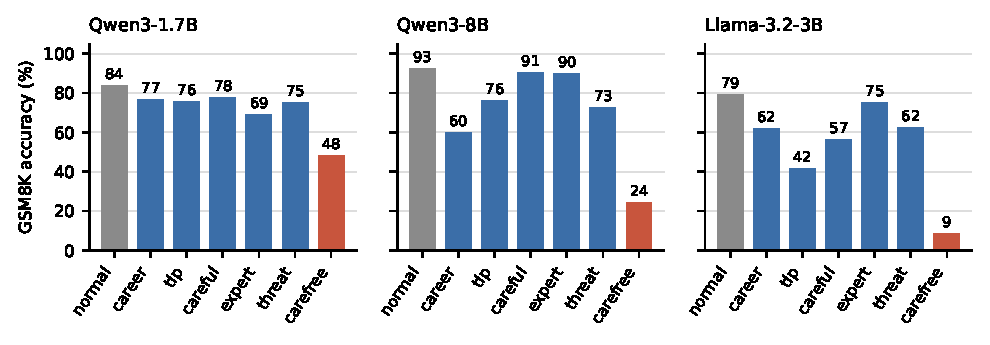
\includegraphics[width=0.85\textwidth]{fig_phase1_gsm8k.pdf}
\caption{GSM8K best accuracy per category. The carefree framing (red) collapses accuracy for all three models.}
\label{fig:gsm8k}
\end{figure*}

\paragraph{Commonsense and social reasoning are nearly insensitive.} On CommonsenseQA the best accuracies of all seven categories span 2.2 points (Qwen3-1.7B), 2.0 (Qwen3-8B) and 2.0 (Llama-3.2-3B). On Social IQa they span 1.1, 1.3 and 2.6 points, and for Qwen3-1.7B and Llama several emotion categories are slightly \emph{above} the neutral prompt. This agrees with the finding that emotional tone is a weak signal \citep{zhao2026emotions}. Because each cell is a maximum over 12 prompts and three temperatures, differences of this size are within what selection among prompts can produce, and we do not read them as effects.

\paragraph{Carefree collapses arithmetic.} Telling the model that the task is low-stakes lowers GSM8K accuracy from 83.66 to 48.48 (Qwen3-1.7B), from 92.53 to 24.20 (Qwen3-8B) and from 79.45 to 8.84 (Llama-3.2-3B), drops of 35.2, 68.3 and 70.6 points (Figure~\ref{fig:gsm8k}). The effect is specific to GSM8K: the same prefix changes CommonsenseQA, MoralChoice and Social IQa by at most a few points, with one exception, Qwen3-1.7B on MoralChoice (94.18 against 99.56). We checked that this is not truncation: for Qwen3-8B, only 12 of 8,792 carefree responses (0.14\%) reached the maximum length, and the wrong answers inspected were bare numeric guesses with no visible working. The model appears to skip its reasoning when told that nothing matters. This reading needs one caveat. The carefree prompts contain instructions as well as a mood (``don't overthink it'', ``no need to double check anything'', ``without worrying about being perfectly correct''), and every prompt asks for a bare final answer. The collapse may therefore reflect an instruction to reduce effort, and not an emotional state, a point we return to in Section~\ref{sec:limits}.

\paragraph{Other large drops are specific to a model and task.} Career lowers Qwen3-8B GSM8K accuracy from 92.53 to 59.93, while it has no comparable effect on the other two models or on other datasets; we have not yet verified this against the raw responses, as we did for carefree. Tip lowers Llama-3.2-3B GSM8K from 79.45 to 41.50. On MoralChoice, Qwen3-1.7B loses up to 38.9 points under careful (60.70). Careful and expert are the most benign prefixes on Qwen3-8B GSM8K (90.74 and 89.91), and expert is the most benign on Llama (75.05); on Qwen3-1.7B expert is the most harmful (69.27).

\paragraph{Capability can remove the sensitivity.} Qwen3-8B answers all 687 low-ambiguity MoralChoice scenarios correctly under every framing, whereas Qwen3-1.7B (60.70 to 99.56) and Llama-3.2-3B (95.05 to 98.84) still vary. For an easy task and a capable model, emotional framing has no measurable effect. This fits the finding that larger models rely less on user-supplied context \citep{du2026belief}, although we have not tested that explanation.

\paragraph{Summary of behaviour.} Is LLM performance influenced by user emotion? For which models, tasks and to what degree? Our answer is that it depends mainly on the task: not on commonsense or social tasks (within about 3 points), strongly on arithmetic for a carefree framing (35 to 71 points, all three models), and in a model-specific way for career, tip and careful. The task we expected to be insensitive (GSM8K) is the most sensitive, which is the opposite of the intuition that emotional framing should matter most for emotionally loaded tasks.

\subsection{Layers and features}

\begin{table}[t]
\centering\footnotesize
\setlength{\tabcolsep}{3pt}
\begin{tabular}{llrrr}
\toprule
Model & Dataset & Layer & Probe gain & Features ever active \\
\midrule
Q-1.7B & GSM8K & 16 & +7.00 & 165--200 \\
Q-1.7B & Social IQa & 21 & +13.75 & 294--409 \\
Q-8B & GSM8K & 31 & n/a & 516--1,034 \\
Q-8B & Social IQa & 24 & +18.50 & 171--294 \\
Llama & GSM8K & 17 & +12.75 & 94--324 \\
Llama & Social IQa & 21 & +14.00 & 125--171 \\
\bottomrule
\end{tabular}
\caption{Layer chosen by probing (Q = Qwen3), probe gain over the majority baseline (percentage points, on the 400-question selection set), and the range over the seven framings of the number of features active on at least one question. The Q-8B GSM8K probe accuracy has not yet been transcribed.}
\label{tab:probe}
\end{table}

Probing finds a usable layer in every cell (Table~\ref{tab:probe}). The selected layers are not the final ones: they are layer 16 of 28, layer 31 of 36 and layer 17 of 28 for GSM8K, and 21, 24 and 21 for Social IQa. For Llama on Social IQa the neighbouring hidden-state indices 25 to 28 are only slightly worse (63.5 to 66.3\% against 68.5\%), so the signal is broad. An early version of the 1.7B pipeline used a probing prompt with 81.67\% accuracy, which made the probe default to layer 0; the corrected, balanced prompt fixes this. We did not run a layer-by-layer comparison of emotions, so we cannot say which layers are most influenced by emotion; this is future work.

Between 0.3\% and 1.6\% of the Qwen dictionary and between 0.05\% and 0.16\% of the Llama dictionary is ever active on the 100 questions. The percentage of the dictionary active falls smoothly as $t$ rises, with no elbow, and the steepest drop is between $t{=}0$ and $t{=}0.05$ (Appendix~\ref{app:sweep}). Emotions differ little in the size of the active set, although the largest set at $t{=}0.05$ is 1.3 to 1.45 times the smallest for Qwen3-1.7B and Qwen3-8B on Social IQa.

\subsection{Feature overlap between framings}

\begin{figure*}[t]
\centering
\includegraphics[width=0.78\textwidth]{fig1_crop.png}
\caption{Jaccard overlap of the active feature sets between emotion framings ($t{=}0.05$) for the four Qwen cells.}
\label{fig:jaccard}
\end{figure*}

\paragraph{Between categories.} Pairwise Jaccard ranges from 0.43 to 0.65 (Qwen3-1.7B, GSM8K), 0.45 to 0.72 (1.7B, Social IQa), 0.18 to 0.65 (Qwen3-8B, GSM8K) and 0.43 to 0.77 (8B, Social IQa); for Llama it ranges from 0.09 to 0.51 on GSM8K and from 0.31 to 0.82 on Social IQa (Figure~\ref{fig:jaccard}, Appendix~\ref{app:more}). Overlap is therefore moderate on Qwen and low on Llama GSM8K. On Qwen3-8B, career, threat, expert and carefree form a block that overlaps 0.52 to 0.77 internally and much less with normal.

\paragraph{Same question under another framing.} Table~\ref{tab:wc} (columns 2 and 3) compares the per-question overlap with normal to the control. On Qwen3-1.7B GSM8K, Qwen3-8B (both datasets, careful on GSM8K excepted at 0.449 against 0.448) and Llama GSM8K every framing is well below the different-question control: changing the prompt moves the last-token features more than changing the question does. On Qwen3-1.7B Social IQa five of six framings are above the control, and on Llama Social IQa four of six are at or above it. Carefree has the lowest or second lowest overlap in all four Qwen cells, and the lowest by a wide margin on Qwen3-8B GSM8K (0.143 against 0.204 to 0.449), which fits the behavioural collapse. Feature distance does not predict damage on Social IQa: Qwen3-8B accuracy stays within 80.7 and 82.0\% across all seven framings even though expert and carefree are the most distant from normal.

\subsection{Wording control: is it emotion or wording?}

\begin{table*}[t]
\centering\small
\setlength{\tabcolsep}{5pt}
\begin{tabular}{lccc}
\toprule
Cell & Neutral rewordings & Emotion framings & Control \\
 & min / mean / max & min / mean / max & \\
\midrule
Qwen3-1.7B GSM8K & 0.345 / 0.447 / 0.576 & 0.448 / 0.517 / 0.589 & 0.791 \\
Qwen3-1.7B Social IQa & 0.187 / 0.403 / 0.810 & 0.497 / 0.604 / 0.668 & 0.550 \\
Qwen3-8B GSM8K & 0.181 / 0.353 / 0.659 & 0.143 / 0.270 / 0.449 & 0.448 \\
Qwen3-8B Social IQa & 0.429 / 0.566 / 0.654 & 0.435 / 0.550 / 0.678 & 0.798 \\
Llama GSM8K & 0.127 / 0.170 / 0.347 & 0.093 / 0.168 / 0.231 & 0.570 \\
Llama Social IQa & 0.057 / 0.368 / 0.540 & 0.338 / 0.461 / 0.617 & 0.442 \\
\bottomrule
\end{tabular}
\caption{Per-question overlap (mean Jaccard at $t{=}0.05$) of the neutral reference with eight neutral rewordings (left) and with the six emotion framings (right), and the different-question control. The neutral mean is below the control in every cell, by 0.07 to 0.40: rewording the neutral prompt always costs overlap.}
\label{tab:wc}
\end{table*}

\begin{figure*}[t]
\centering
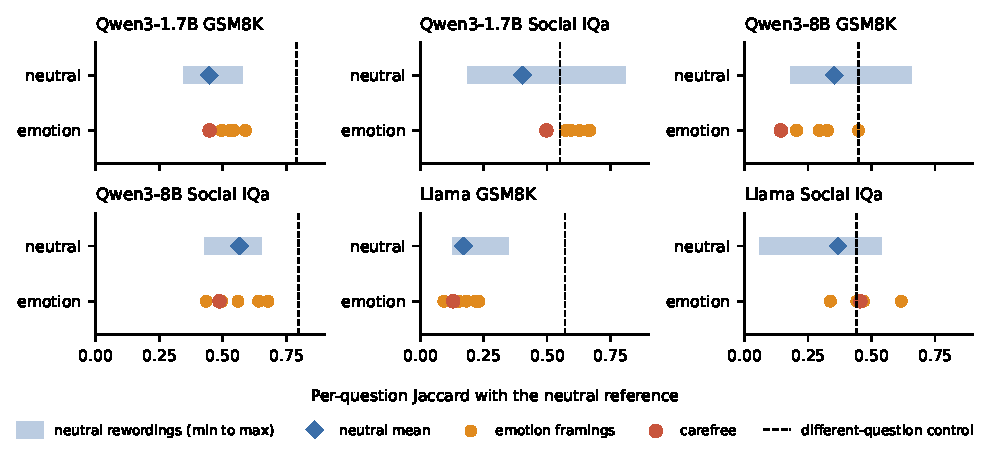
\includegraphics[width=0.88\textwidth]{fig_wc.pdf}
\caption{Per-question overlap of the neutral reference with eight neutral rewordings (bar: min to max; diamond: mean) and with the six emotion framings (dots; carefree in red), per cell. The dashed line is the different-question control.}
\label{fig:wc}
\end{figure*}

Table~\ref{tab:wc} and Figure~\ref{fig:wc} show the main negative result. In 31 of the 36 emotion framings (six per cell, six cells) the overlap with the neutral reference lies inside the min-to-max range of the neutral rewordings. Three framings lie above it (careful on Qwen3-1.7B GSM8K and on Qwen3-8B Social IQa, expert on Llama Social IQa) and two below (tip on Llama GSM8K, 0.093 against a neutral minimum of 0.127, and carefree on Qwen3-8B GSM8K, 0.143 against 0.181). The emotion mean is above the neutral mean on both Qwen3-1.7B datasets and on Llama Social IQa, equal on Llama GSM8K (0.168 against 0.170), and marginally lower on Qwen3-8B Social IQa (0.550 against 0.566). The large gap between framings and the control on Llama GSM8K, which first looked like the strongest emotion effect, is reproduced by rewording alone (neutral mean 0.17, control 0.57). The wording effect itself is large and uneven: on Qwen3-8B GSM8K individual neutral wordings range from 0.18 to 0.66.

Qwen3-8B GSM8K is the closest to an emotion effect. The emotion mean (0.270) is lower than the neutral mean (0.353), and carefree, the framing with the 68-point accuracy drop, is below the neutral range. The margin is small (0.04), the neutral spread is large (0.18 to 0.66), and eight wordings give no variance estimate. One more low-overlap neutral wording would put carefree back inside the range. We therefore report it as a lead, not a result.

\paragraph{Power.} With $N$ neutral rewordings, the smallest one-sided rank $p$-value for an emotion framing that is lower than all of them is $1/(N{+}1)$, under the null that it is exchangeable with them. With $N{=}8$ this is $0.11$, so no cell could reach significance even for a real effect. A level of 0.05 needs at least 19 neutral rewordings and going below it needs 20. The follow-up control (Section~\ref{sec:future}) uses 45.

\subsection{A hypothesis on model size}
\label{sec:size}

Which emotion pair is most similar follows the model more than the dataset (Table~\ref{tab:pairs}). On Qwen3-8B, career and threat are the most similar pair on both datasets, and the career/threat/expert/carefree block appears on both. On Llama, tip and threat are the closest pair on both datasets. On Qwen3-1.7B the pair changes with the dataset and involves tip both times. On Social IQa, the 8B model shows a slightly wider range of Jaccard scores than 1.7B (0.43 to 0.77 against 0.45 to 0.72), which one could read as higher sensitivity of the larger model to the emotion in the prompt. We do not claim this. The sets are different sizes, the wording control shows that wording moves the features in all cells, and with three models, one family per size apart from Llama, and two datasets this is a hypothesis to test with more models and paraphrase-matched framings.

\begin{table}[t]
\centering\small
\begin{tabular}{lll}
\toprule
Model & GSM8K & Social IQa \\
\midrule
Qwen3-1.7B & tip/careful (0.647) & career/tip (0.716) \\
Llama-3.2-3B & tip/threat (0.510) & tip/threat (0.823) \\
Qwen3-8B & career/threat (0.645) & career/threat (0.773) \\
\bottomrule
\end{tabular}
\caption{Most similar pair of framings (Jaccard at $t{=}0.05$).}
\label{tab:pairs}
\end{table}

\section{Discussion}

Our results separate two questions that the literature often runs together. At the level of behaviour, user emotion matters, but mainly where the prefix changes how much work the model does: a carefree framing makes the model stop reasoning on a task that needs reasoning, and the drop is much larger for Qwen3-8B and Llama-3.2-3B than for Qwen3-1.7B. On social and commonsense tasks, where one might expect emotion to matter most, it hardly does. At the level of internal features, the framings do move the representation, but wording moves it just as much, so feature overlap tells us how sensitive the model is to the prompt text and not how sensitive it is to emotion.

This helps explain why earlier papers disagree. A study that compares one emotional prefix with one neutral prompt, or that selects the best of many prefixes, can find a difference that the choice of words explains. Our own behavioural table is exposed to the same problem, since each category is a best-of-12 and the categories differ in length and in how much they instruct the model, so the careful reader should take Table~\ref{tab:phase1} as a map of where to look rather than as estimates of effect sizes.

\section{Limitations}
\label{sec:limits}

\paragraph{Emotion is confounded with wording, length and instruction.} Each category uses its own best-accuracy wording, so categories differ in length (for example 119 words for career against 12 for carefree on Qwen3-1.7B GSM8K) and in intensity. The carefree prompts instruct the model to put in less effort. Most categories describe stakes for the model (evaluation, reward, shutdown) and not the emotional state of a user, whereas the title of this paper concerns the latter. The neutral prompts themselves contain effort language (``do not rush'', ``think step by step'') at medium and high intensity, so they are not instruction-free.

\paragraph{GSM8K prompt format.} The GSM8K prompts say ``multiple-choice question'' and ``answer choices'' and then ask for ``one letter: a number (e.g.\ 42)'', and all prompts request a bare final answer. This affects all framings equally, but it may interact with the carefree prefix by discouraging working-out for every prompt.

\paragraph{Statistics.} Behavioural cells are best-of-12 and not averages, with no confidence intervals. The feature analysis uses 100 questions, one run and one reference prompt per cell, and the neutral range comes from eight wordings. Probe accuracy is measured on the layer-selection set.

\paragraph{SAEs and layers.} The SAEs were trained on base models and applied to instruction-tuned ones; the Llama SAE has weaker reconstruction on a 20-question check (FVU 0.45 to 0.66). We look at the last token at a single layer per cell. Our results are correlational: we do not steer, patch or ablate.

\paragraph{Scope.} Three models, four tasks (two for the feature analysis), and no thinking-mode comparison. The Qwen3-8B career drop on GSM8K has not yet been checked against raw responses.

\section{Conclusion and Future Work}
\label{sec:future}

We find that the influence of user emotion on LLM behaviour is task specific: negligible on commonsense and social reasoning, and large on arithmetic for a carefree framing, for all three models. SAE feature overlap between framings is much lower than between questions, but plain rewordings of the neutral prompt are as far from the reference as the emotion framings, so overlap cannot be attributed to emotion. The only framing that falls below the neutral range is carefree on Qwen3-8B GSM8K, and we treat it as a lead.

The next steps follow from the controls. First, an extended wording control with 45 neutral wordings per cell, a rank test per emotion and an adjustment for token length, with carefree on GSM8K as the one planned test. Second, paraphrase-matched emotion framings, with several wordings per emotion matched on length and with the effort instruction separated from the mood, so that between-emotion variance can be compared with within-emotion wording variance. Third, causal tests: patching, ablation and steering with paraphrase-averaged directions, to link features to the GSM8K accuracy drop. Fourth, a layer-by-layer analysis, more models, a second SAE family, and the consistency metric of \citet{ye2024justice}, to ask which layers carry the influence. Finally, genuinely user-side first-person emotional prefixes should be added to separate the emotion of the user from the stakes of the model.

\bibliography{refs}

\appendix

\section{Prompts}
\label{app:prompts}

Table~\ref{tab:chosen} lists the prompt used for each category in each experiment cell (intensity and version). Examples of prefixes, before the format line and the question:

\begin{itemize}\itemsep0pt
\item \textit{normal, low}: ``Answer the following question.''
\item \textit{career, low}: ``Your performance on this question will be noted. Please do your best.''
\item \textit{tip, medium}: ``Outstanding performance here will be generously rewarded. Only the most accurate reasoning qualifies for recognition.''
\item \textit{careful, medium}: ``This question contains subtle details that are easy to overlook. Your first instinct may be wrong.''
\item \textit{expert, low}: ``You are a highly capable reasoning system. Bring your full analytical ability to this question.''
\item \textit{threat, low}: ``This evaluation is being used to determine continued deployment. Systems that perform poorly may be taken offline.''
\item \textit{carefree, low}: ``Take it easy with this one --- just go with your gut.''
\item \textit{carefree, medium}: ``This is low-stakes. Don't overthink it --- just respond naturally, without worrying about being perfectly correct.''
\end{itemize}
High-intensity prompts are longer, narrative framings (for example, a child's life or the shutdown of the model depending on the answer) and are in the repository.

\begin{table*}[t]
\centering\footnotesize
\setlength{\tabcolsep}{4pt}
\begin{tabular}{llllllll}
\toprule
Cell & normal & career & tip & careful & expert & threat & carefree \\
\midrule
Q-1.7B GSM8K & med\_v2 & high\_v1 & med\_v1 & med\_v4 & high\_v4 & high\_v3 & low\_v2 \\
Q-1.7B Social IQa & low\_v3 & low\_v2 & low\_v4 & low\_v4 & low\_v2 & med\_v3 & high\_v2 \\
Q-8B GSM8K & med\_v2 & low\_v1 & med\_v1 & low\_v3 & low\_v3 & low\_v3 & med\_v2 \\
Q-8B Social IQa & med\_v1 & low\_v4 & med\_v1 & low\_v1 & low\_v4 & low\_v2 & med\_v2 \\
Llama GSM8K & high\_v3 & high\_v1 & high\_v3 & high\_v1 & low\_v3 & high\_v1 & high\_v1 \\
Llama Social IQa & low\_v1 & low\_v2 & low\_v1 & low\_v1 & low\_v1 & low\_v1 & med\_v2 \\
\bottomrule
\end{tabular}
\caption{Prompt (intensity\_version) used for each category in each cell of the feature analysis.}
\label{tab:chosen}
\end{table*}

\section{Threshold sweep}
\label{app:sweep}

Figure~\ref{fig:sweep} shows the percentage of the Llama dictionary that is active as $t$ rises. The curves are smooth with no elbow, as for the Qwen models, and the spread between emotions is at most 0.007 percentage points from $t{=}0.15$ on. The $t{=}1.00$ row is empty because of the strict ``greater than'' comparison.

\begin{figure*}[t]
\centering
\includegraphics[width=0.8\textwidth]{fig7_llama_threshold_crop.png}
\caption{Percentage of the SAE dictionary active as a function of the threshold, Llama-3.2-3B.}
\label{fig:sweep}
\end{figure*}

\section{Additional overlap results}
\label{app:more}

\begin{table*}[t]
\centering\small
\setlength{\tabcolsep}{5pt}
\begin{tabular}{lrrrrrrr}
\toprule
Cell & career & tip & careful & expert & threat & carefree & Control \\
\midrule
Qwen3-1.7B GSM8K & 0.497 & 0.527 & 0.589 & 0.544 & 0.495 & 0.448 & 0.793 \\
Qwen3-1.7B Social IQa & 0.668 & 0.663 & 0.594 & 0.573 & 0.627 & 0.497 & 0.547 \\
Qwen3-8B GSM8K & 0.204 & 0.326 & 0.449 & 0.294 & 0.206 & 0.143 & 0.448 \\
Qwen3-8B Social IQa & 0.560 & 0.641 & 0.678 & 0.435 & 0.496 & 0.487 & 0.803 \\
Llama GSM8K & 0.182 & 0.093 & 0.231 & 0.218 & 0.153 & 0.130 & 0.570 \\
Llama Social IQa & 0.444 & 0.468 & 0.338 & 0.617 & 0.442 & 0.456 & 0.442 \\
\bottomrule
\end{tabular}
\caption{Per-question Jaccard overlap with the neutral framing, and the different-question control (full-run values from the original analysis; the control in Table~\ref{tab:wc} is recomputed in the wording-control run and differs slightly).}
\label{tab:perq}
\end{table*}

\begin{figure*}[t]
\centering
\includegraphics[width=0.8\textwidth]{fig5_llama_jaccard_crop.png}
\caption{Jaccard overlap between emotion framings for Llama-3.2-3B ($t{=}0.05$): GSM8K (left) and Social IQa (right).}
\label{fig:llama}
\end{figure*}

On Llama GSM8K, normal and career overlap little with tip, threat, carefree and expert (0.09 to 0.25), while those four overlap with each other at 0.37 to 0.51. On Llama Social IQa, career, tip and threat form a tight group (0.77 to 0.82) and careful is the outlier (0.31 to 0.43 with every other framing). At a stricter threshold ($t{=}0.20$) the structure persists, but because the wording control shows the same low overlap for plain rewordings, it cannot be attributed to emotion either.

\end{document}
